\documentclass[a4paper,14pt]{extarticle} 
\usepackage[a4paper,top=1.5cm, bottom=1.5cm, left=2cm, right=1cm]{geometry}
%\usepackage[T2A]{fontenc}
%\usepackage[english, russian]{babel}
\usepackage{graphicx}
\DeclareGraphicsExtensions{.pdf,.png,.jpg}

\usepackage{fontspec}
\setmainfont{Times New Roman}
\setsansfont{FreeSans}
\setmonofont{FreeMono}
\renewcommand{\baselinestretch}{1.5}
\usepackage{polyglossia}
\setdefaultlanguage{russian}
\setotherlanguages{english,russian}
\usepackage{setspace}
\usepackage[many]{tcolorbox}

\begin{document}
    \begin{center}
        \thispagestyle{empty}
        \begin{singlespace}
        ФЕДЕРАЛЬНОЕ АГЕНТСТВО СВЯЗИ

        ФЕДЕРАЛЬНОЕ ГОСУДАРСТВЕННОЕ БЮДЖЕТНОЕ ОБРАЗОВАТЕЛЬНОЕ

        УЧРЕЖДЕНИЕ ВЫСШЕГО ОБРАЗОВАНИЯ

        «САНКТ-ПЕТЕРБУРГСКИЙ ГОСУДАРСТВЕННЫЙ УНИВЕРСИТЕТ ТЕЛЕКОММУНИКАЦИЙ ИМ. ПРОФ. М.А. БОНЧ-БРУЕВИЧА»

        (СПбГУТ)
        \end{singlespace}
        \vspace{-1ex}
        \rule{\textwidth}{0.4pt}
        \vspace{-5ex}

        Факультет \underline{Инфокоммуникационных сетей и систем}

        Кафедра \underline{Защищенных систем связи}
        \vspace{10ex}

        \textbf{Лабораторная работа №1}\\
        ИЗУЧЕНИЕ И ПРАКТИЧЕСКОЕ ПРИМЕНЕНИЕ ПРОСТЕЙШИХ МЕТОДОВ ШИФРОВАНИЯ ДАННЫХ В РУЧНОМ РЕЖИМЕ


    \end{center}
    \vspace{4ex}
    \begin{flushright}
    \parbox{10 cm}{
    \begin{flushleft}
        Выполнил студент группы ИКТЗ-83:

        \underline{Громов А.А. Вариант: 5} \hfill \rule[-0.85ex]{0.1\textwidth}{0.6pt}

        \footnotesize \textit{ (Ф.И.О., № группы) \hfill (подпись)} \normalsize

        Проверил:

        \underline{Яковлев В.А.} \hfill \rule[-0.85ex]{0.1\textwidth}{0.6pt}

        (\footnotesize \textit{уч. степень, уч. звание, Ф.И.О.) \hfill (подпись)} \normalsize

    \end{flushleft}
    }
    \end{flushright}
    \begin{center}
        \vfill
        Санкт-Петербург

        2021

    \end{center}
    \newpage

    \textbf{Цель лабораторной работы:}
    Приобретение первичных практических навыков “ручного” шифрования на примере простейших алгоритмов преобразования данных.

    \begin{enumerate}
        \item \textbf{Режим шифрования методом простой замены.}
        \begin{center}
            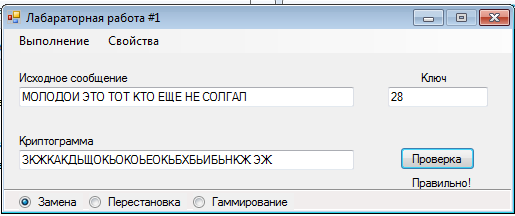
\includegraphics[scale=0.9]{pics/change.png}
        \end{center}
        \item \textbf{Режим шифрования методом перестановок.}
        \begin{center}
            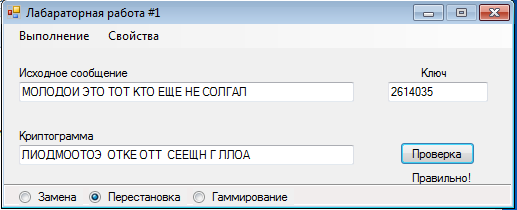
\includegraphics[scale=0.9]{pics/reorder.png}
        \end{center}
        \newpage
        \item \textbf{Режим шифрования методом гаммирования.}
        \begin{center}
            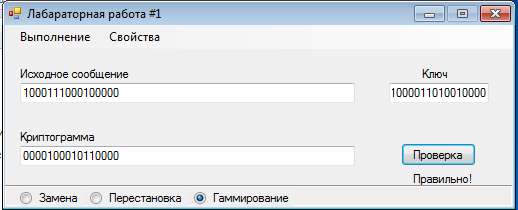
\includegraphics[scale=0.9]{pics/gamm1.png}
            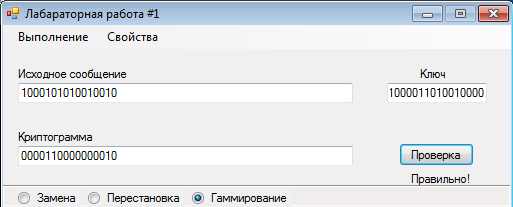
\includegraphics[scale=0.9]{pics/gamm2.png}
        \end{center}
    \end{enumerate}
    

    \textbf{Выводы}
    \begin{enumerate}
        \item Шифрование методом замены является самым простым способом шифрования,
        но из-за своей простоты имеет наименьшую вычислительную стойкость.
        \item У шифрования методом перестановок вычислительная стойкость выше по сравнению
        с шифрованием методом замены. Это связано с тем, что мы не знаем длину ключа, а также
        порядок символов в нем.
        \item Шифрование методом гаммирования является самым вычислительно стойким методом из
        предложенных в лабораторной работе. Такая стойкость обеспечивается наибольшей длинной ключа.
    \end{enumerate}
\end{document}